\documentclass[fleqn,11pt, french, ceqn]{article}

\setlength{\parindent}{0pt}
\setlength{\parskip}{1em}

\usepackage[T1]{fontenc}
\usepackage[utf8]{inputenc}
\usepackage{lmodern}
\usepackage[a4paper, scale=0.8]{geometry}
\usepackage[francais]{babel}
\usepackage{subfiles}
\usepackage{tabularx}
\usepackage{url}
\usepackage{xcolor}
\usepackage{multicol}
\usepackage{pbox}
\usepackage[hidelinks]{hyperref}
\usepackage{subcaption}

\usepackage{pdfpages}

\usepackage{tikz}

\usepackage{graphicx}

\usepackage{algorithm}
\usepackage{algorithmic}

\usepackage{array}
\usepackage{amsthm}
\usepackage{amssymb}
\usepackage{amsmath}
\usepackage{bbold}
\theoremstyle{plain}
\newtheorem{thm}{Théorème}
\newtheorem{prop}{Proposition}
\newtheorem{coro}{Corollaire}
\newtheorem{lem}{Lemme}

\theoremstyle{definition}
\newtheorem{defn}{Définition}
\newtheorem{exemple}{Exemple}


\theoremstyle{remark}
\newtheorem{rem}{Remarque}
\newtheorem{exercice}{Exercice}
\newtheorem{quest}{Question}

%% Ensemble usuels 

\newcommand{\rel}{\mathbb{Z}}
\newcommand{\nat}{\mathbb{N}}
\newcommand{\rat}{\mathbb{Q}}
\newcommand{\real}{\mathbb{R}}
\newcommand{\complex}{\mathbb{C}}

\newcommand{\Esp}{\mathbb{E}}

\newcommand{\Z}{\rel}
\newcommand{\N}{\nat}
\newcommand{\Q}{\rat}
\newcommand{\R}{\real}
%\newcommand{\C}{\complex}
\newcommand{\ZZ}[1]{\relmod{#1}}

\newcommand{\unit}{\mathbb{U}}
\newcommand{\relmod}[1]{\rel/#1\rel}
\newcommand{\realcontinous}{\mathcal C \left(\real, \real\right)}

\newcommand{\gradient}{\nabla}

%% Notations ephémères
\newcommand{\Arond}{\mathcal A}
\newcommand{\Brond}{\mathcal B}
\newcommand{\Crond}{\mathcal C}
\newcommand{\Drond}{\mathcal D}
\newcommand{\Erond}{\mathcal E}
\newcommand{\Frond}{\mathcal F}
\newcommand{\Grond}{\mathcal G}
\newcommand{\Hrond}{\mathcal H}
\newcommand{\Irond}{\mathcal I}
\newcommand{\Jrond}{\mathcal J}
\newcommand{\Krond}{\mathcal K}
\newcommand{\Lrond}{\mathcal L}
\newcommand{\Mrond}{\mathcal M}
\newcommand{\Nrond}{\mathcal N}
\newcommand{\Orond}{\mathcal O}
\newcommand{\Prond}{\mathcal P}
\newcommand{\Qrond}{\mathcal Q}
\newcommand{\Rrond}{\mathcal R}
\newcommand{\Srond}{\mathcal S}
\newcommand{\Trond}{\mathcal T}
\newcommand{\Urond}{\mathcal U}
\newcommand{\Vrond}{\mathcal V}
\newcommand{\Wrond}{\mathcal W}
\newcommand{\Xrond}{\mathcal X}
\newcommand{\Yrond}{\mathcal Y}
\newcommand{\Zrond}{\mathcal Z}

\newcommand{\Abf}{\mathbf A}
\newcommand{\Bbf}{\mathbf B}
\newcommand{\Cbf}{\mathbf C}
\newcommand{\Dbf}{\mathbf D}
\newcommand{\Ebf}{\mathbf E}
\newcommand{\Fbf}{\mathbf F}
\newcommand{\Gbf}{\mathbf G}
\newcommand{\Hbf}{\mathbf H}
\newcommand{\Ibf}{\mathbf I}
\newcommand{\Jbf}{\mathbf J}
\newcommand{\Kbf}{\mathbf K}
\newcommand{\Lbf}{\mathbf L}
\newcommand{\Mbf}{\mathbf M}
\newcommand{\Nbf}{\mathbf N}
\newcommand{\Obf}{\mathbf O}
\newcommand{\Pbf}{\mathbf P}
\newcommand{\Qbf}{\mathbf Q}
\newcommand{\Rbf}{\mathbf R}
\newcommand{\Sbf}{\mathbf S}
\newcommand{\Tbf}{\mathbf T}
\newcommand{\Ubf}{\mathbf U}
\newcommand{\Vbf}{\mathbf V}
\newcommand{\Wbf}{\mathbf W}
\newcommand{\Xbf}{\mathbf X}
\newcommand{\Ybf}{\mathbf Y}
\newcommand{\Zbf}{\mathbf Z}


%% Topologie

\newcommand{\Topo}{\mathcal{O}}
\newcommand{\Int}[1]{\mathring{#1}}
\newcommand{\Adh}[1]{\overline{#1}}
\newcommand{\Fr}{\mathit{Fr}}
% Espace métriques
\newcommand{\Bo}{\mathcal{B}}
\newcommand{\Bf}{\bar{\mathcal{B}}}

\newcommand{\vertiii}[1]{{\left\vert\kern-0.25ex\left\vert\kern-0.25ex\left\vert #1 
    \right\vert\kern-0.25ex\right\vert\kern-0.25ex\right\vert}}


\newcommand{\congr}{\equiv}
\newcommand{\Vois}{\mathcal{V}}

\newcommand{\SL}{\mathbf{SL}}
\newcommand{\SO}{\mathbf{SO}}
\newcommand{\Bij}{\mathcal Bij}
\newcommand{\Perm}{\mathfrak{S}}

\newcommand{\dd}{\mathrm d}

\newcommand{\onebb}{1\!\!1}

\newcommand{\parts}[1]{\mathcal{P}\left(#1\right)}

\newcommand{\abs}[1]{\left|#1\right|}
\newcommand{\norm}[1]{\left|\left|#1\right|\right|}


\newcommand{\kev}{$\mathbb{K}$-ev }
\newcommand{\Aut}{\mathcal{A}ut}
\newcommand{\signa}{\epsilon}
\newcommand{\inv}[1]{\frac{1}{#1}}

\newcommand{\ds}{\displaystyle}
\newcommand{\fact}[1]{#1~!}

\newcommand{\card}[1]{\left| #1\right|}
%\newcommand{\card}[1]{\##1}
%\newcommand{\card}[1]{\mathrm{Card}\left(#1\right)}

\newcommand{\set}[1]{\left\{ #1\right\}}
\newcommand{\eng}[1]{\left< #1\right>}
\newcommand{\interclosed}[1]{\left[ #1\right]}
\newcommand{\interopend}[1]{\left] #1 \right[}
\newcommand{\im}{\mathrm{Im}}
\renewcommand{\geq}{\geqslant}
\renewcommand{\leq}{\leqslant}
\renewcommand{\iff}{\Leftrightarrow}

\newcommand{\longto}{\longrightarrow}

\newcommand{\Id}{\mathit{Id}}
\newcommand{\Ind}{\mathbb{1}}

\newcommand{\lpar}{\left(}
\newcommand{\rpar}{\right)}

\newcommand{\follows}{\sim}



%% Graphes

\newcommand{\Ger}{\mathbb G}

%% Proba

\newcommand{\Proba}{\mathbb P}
\newcommand{\1}{\matbb 1}
\newcommand{\Bin}{\mathcal B}

\newcommand{\NP}{\mathcal{NP}}
\newcommand{\PP}{\mathcal{P}}


\title{Adam: A method for stochastic Optimization}
\author{Maxime \textsc{Darrin}}


\begin{document}
	\maketitle
	\tableofcontents

	\newpage
	
	\section{Introduction}
	
	Adam est une méthode originellement proposée par en 2015 par D.P Kingma et J. Lei Ba à la conférence ICLR. C'est une méthode d'optimisation du premier ordre introduisant une méthode de conservation du moment d'inertie (\emph{momentum} en anglais) couplée à un \emph{learning rate} adaptatif.
	
	Il reprend le principe de l'\emph{adaptative learning rate} utilisé par \emph{Adadelta\cite{adadelta}} et \emph{RMSProp\cite{rmsprop}}, c'est à dire qu'il conserve une moyenne temporelle (l'importance du passé diminue exponentiellement avec le temps) du carré des gradients précédemment calculés de sorte à conserve une notion de variance des-dits gradients.
		
	A cela, il ajoute une conservation de l'inertie. Il estime la moyenne des gradients (simples cette fois-ci) précédemment calculés, de même que précédemment en accordant plus d'importance aux observations récentes qu'au passé en faisant diminuer exponentiellement avec le temps l'importance du passé. L'idée est de conserver une notion de moyenne de la pente courante et de continuer à aller "un peu" dans les directions prises dans le passé.
	
	Ces deux propriétés simulent en fait la trajectoire qu'une boule qui roulerait (avec de la friction) sur la surface d'erreur, aurait.
	
	Dans un premier temps 
	
	
	\section{Principes et justification}
	
	\subsection{\emph{Adaptavie learning rate}}
	
	Tout d'abord, on rappelle la méthode \emph{RMS Prop} proposée par Geoff Hinton\cite{rmsprop}. On maintient une estimation de la moyenne des carrés des coordonnées des gradients, c'est à dire de la variance non centrée. Et on l'utilise pour adapter le \emph{learning rate}. Dans la suite on notera $g_t$ le vecteur des gradient calculé au temps $t$ et l'application des carrés se fait coordonnées à coordonnées.
	
	\begin{figure}[H]
		\centering
		\begin{align*}
			E[g^2]_t &= 0.9 E[g^2]_{t-1} + 0.1 g^2_t \\ 
			\theta_{t+1} &= \theta_{t} - \dfrac{\eta}{\sqrt{E[g^2]_t + \epsilon}} g_{t} 
		\end{align*}
		\caption{Mise à jour pour \emph{RMSProp}}
	\end{figure}

	\emph{Adam} reprend ce principe de manière plus générale: pour $\beta_2 \in [0,1]$ , on calcule $v_t = \beta_2 b_{t-1} +  (1-\beta_2)g_t^2$.
	
	Les auteurs notes que cet estimateur est biaisé vers $0$ en particulier lorsque $\beta_2$ est proche de $1$. Ils proposent alors de redresser cet estimateur pour le rendre non biaisé:
	
	\begin{align*}
		\hat{v}_t &= \dfrac{v_t}{1 - \beta^t_2}
	\end{align*}
	
	\subsection{Inertie}
	
	En plus de l'adaptation du \emph{learning rate} \emph{Adam} conserve de l'inertie dans sa descente de gradient, pour ce faire maintien une estimation de la moyenne des prédédents gradients, pour $\beta_1$: $m_t = \beta_1 m_{t-1} + (1-\beta_1) g_t$
	
	Néanmoins, comme pour la variance cet estimateur de la moyenne est biaisé. On le redresse de la même manière:
	\begin{align*}
		\hat{m}_t &= \dfrac{m_t}{1 - \beta^t_1}
	\end{align*}
	
	\subsection{Couplage des deux grandeurs}
	
	En couplant les estimations de l'inertie et de la variance on obtient une règle de mise à jour qui adapte le \emph{learning rate} et qui simule l'inertie de descente:
	\begin{center}
	$
		\begin{array}{ll}
		m_t = \beta_1 m_{t-1} + (1-\beta_1) g_t & \hat{m}_t = \dfrac{m_t}{1 - \beta^t_1} \\
		v_t = \beta_2 b_{t-1} +  (1-\beta_2)g_t^2 & \hat{v}_t = \dfrac{v_t}{1 - \beta^t_2} \\
		
		\theta_{t+1} = \theta_{t} - \dfrac{\eta}{\sqrt{\hat{v}_t} + \epsilon} \hat{m}_t & \\
		\end{array}
	$
	\end{center}

	On peut alors analyser la règle de mise à jour. On a $\Delta_{t+1} = \theta_{t+1} - \theta_{t} = - \frac{\eta}{\sqrt{\hat{v}_t} + \epsilon} \hat{m}_t$. Ainsi, la taille d'un pas de la descente de gradient est de l'ordre de $\frac{\hat{m}_t}{\sqrt{\hat{v}_t}}$, c'est à dire la moyenne sur le carré de la variance non centrée qui est ici le ratio signal bruit. Et on voit donc, que lorsque ce ratio est faible, c'est à dire que le bruit est élevé -- et donc l'incertitude sur la direction à suivre, on fait des pas plus petits ce qui correspond intuitivement à ce que l'on voudrait faire. En effet, cette incertitude est en général d'autant plus grande qu'on se rapproche d'un minimum (local ou non). Au contraire, lorsque ce ratio est élevé, on peut se permettre de faire de plus grands pas sans risques.
	
	\section{Algorithme ADAM}
	
	\begin{algorithm}[H]
		\begin{algorithmic}
			\REQUIRE{$\eta$ stepsize}
			\REQUIRE{$\beta_1, \beta_2, \epsilon \in  [0,1]$}
			\REQUIRE{$f(\theta)$ loss to minimize}
			
			\STATE{Initialize $\theta_0$}
			\STATE{Initialize $m_0, v_0$ to zeros vectors}
			\STATE{$t \gets 0$}
			
			\WHILE{$\theta_n$ has not converged}
				\STATE{$g_t \gets \gradient_{\theta_t} f(\theta_t)$}
				\STATE{$m_t \gets \beta_1 m_{t-1} + (1-\beta_1) g_t$}
				\STATE{$v_t \gets \beta_2 b_{t-1} +  (1-\beta_2)g_t^2$}
				\STATE{$\hat{m}_t \gets \dfrac{m_t}{1 - \beta^t_1}$}
				\STATE{$ \hat{v}_t \gets \dfrac{v_t}{1 - \beta^t_2}$}
				
				\STATE{$\theta_{t+1} \gets \theta_{t} - \dfrac{\eta}{\sqrt{\hat{v}_t} + \epsilon} \hat{m}_t$}
				\STATE{$t \gets t +1$}
			\ENDWHILE
		\end{algorithmic}
	\caption{ Adam}
	\end{algorithm}
	
	\section{Résultats empiriques}
	
	\subsection{Comportement sur des problèmes jouets}
	
	On commence par tester l'algorithme présenté pour optimiser des fonctions jouets et on compare les résultats obtenus avec une descente de gradient usuelle.
	
	\begin{figure}[H]
		\centering
		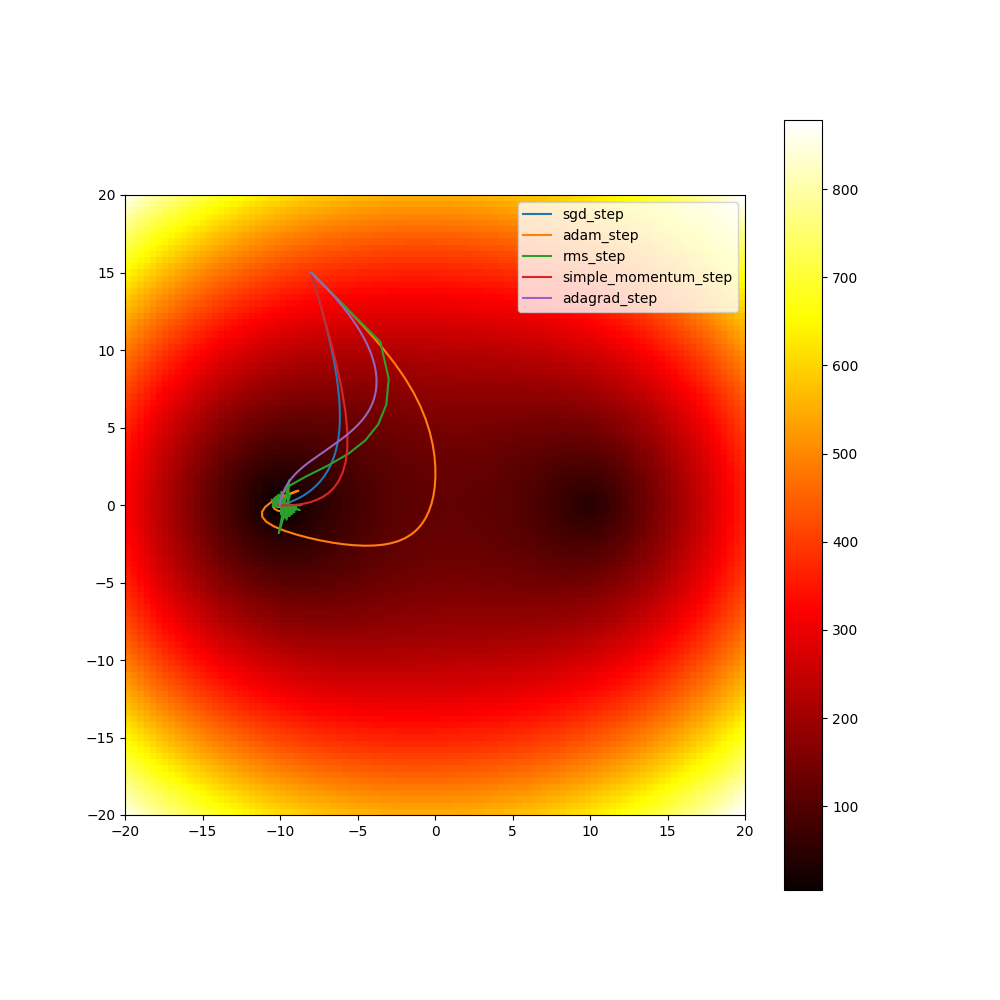
\includegraphics[scale=0.5]{../gdsvm/exports/adam-rms-sgd.png}
		\caption{Comparaison entre adam (vert), sgd (bleu) et RMSProp (rose)}
	\end{figure}
	
	\subsection{Résultats sur MNIST}
	
		\begin{figure}[H]
		\centering
		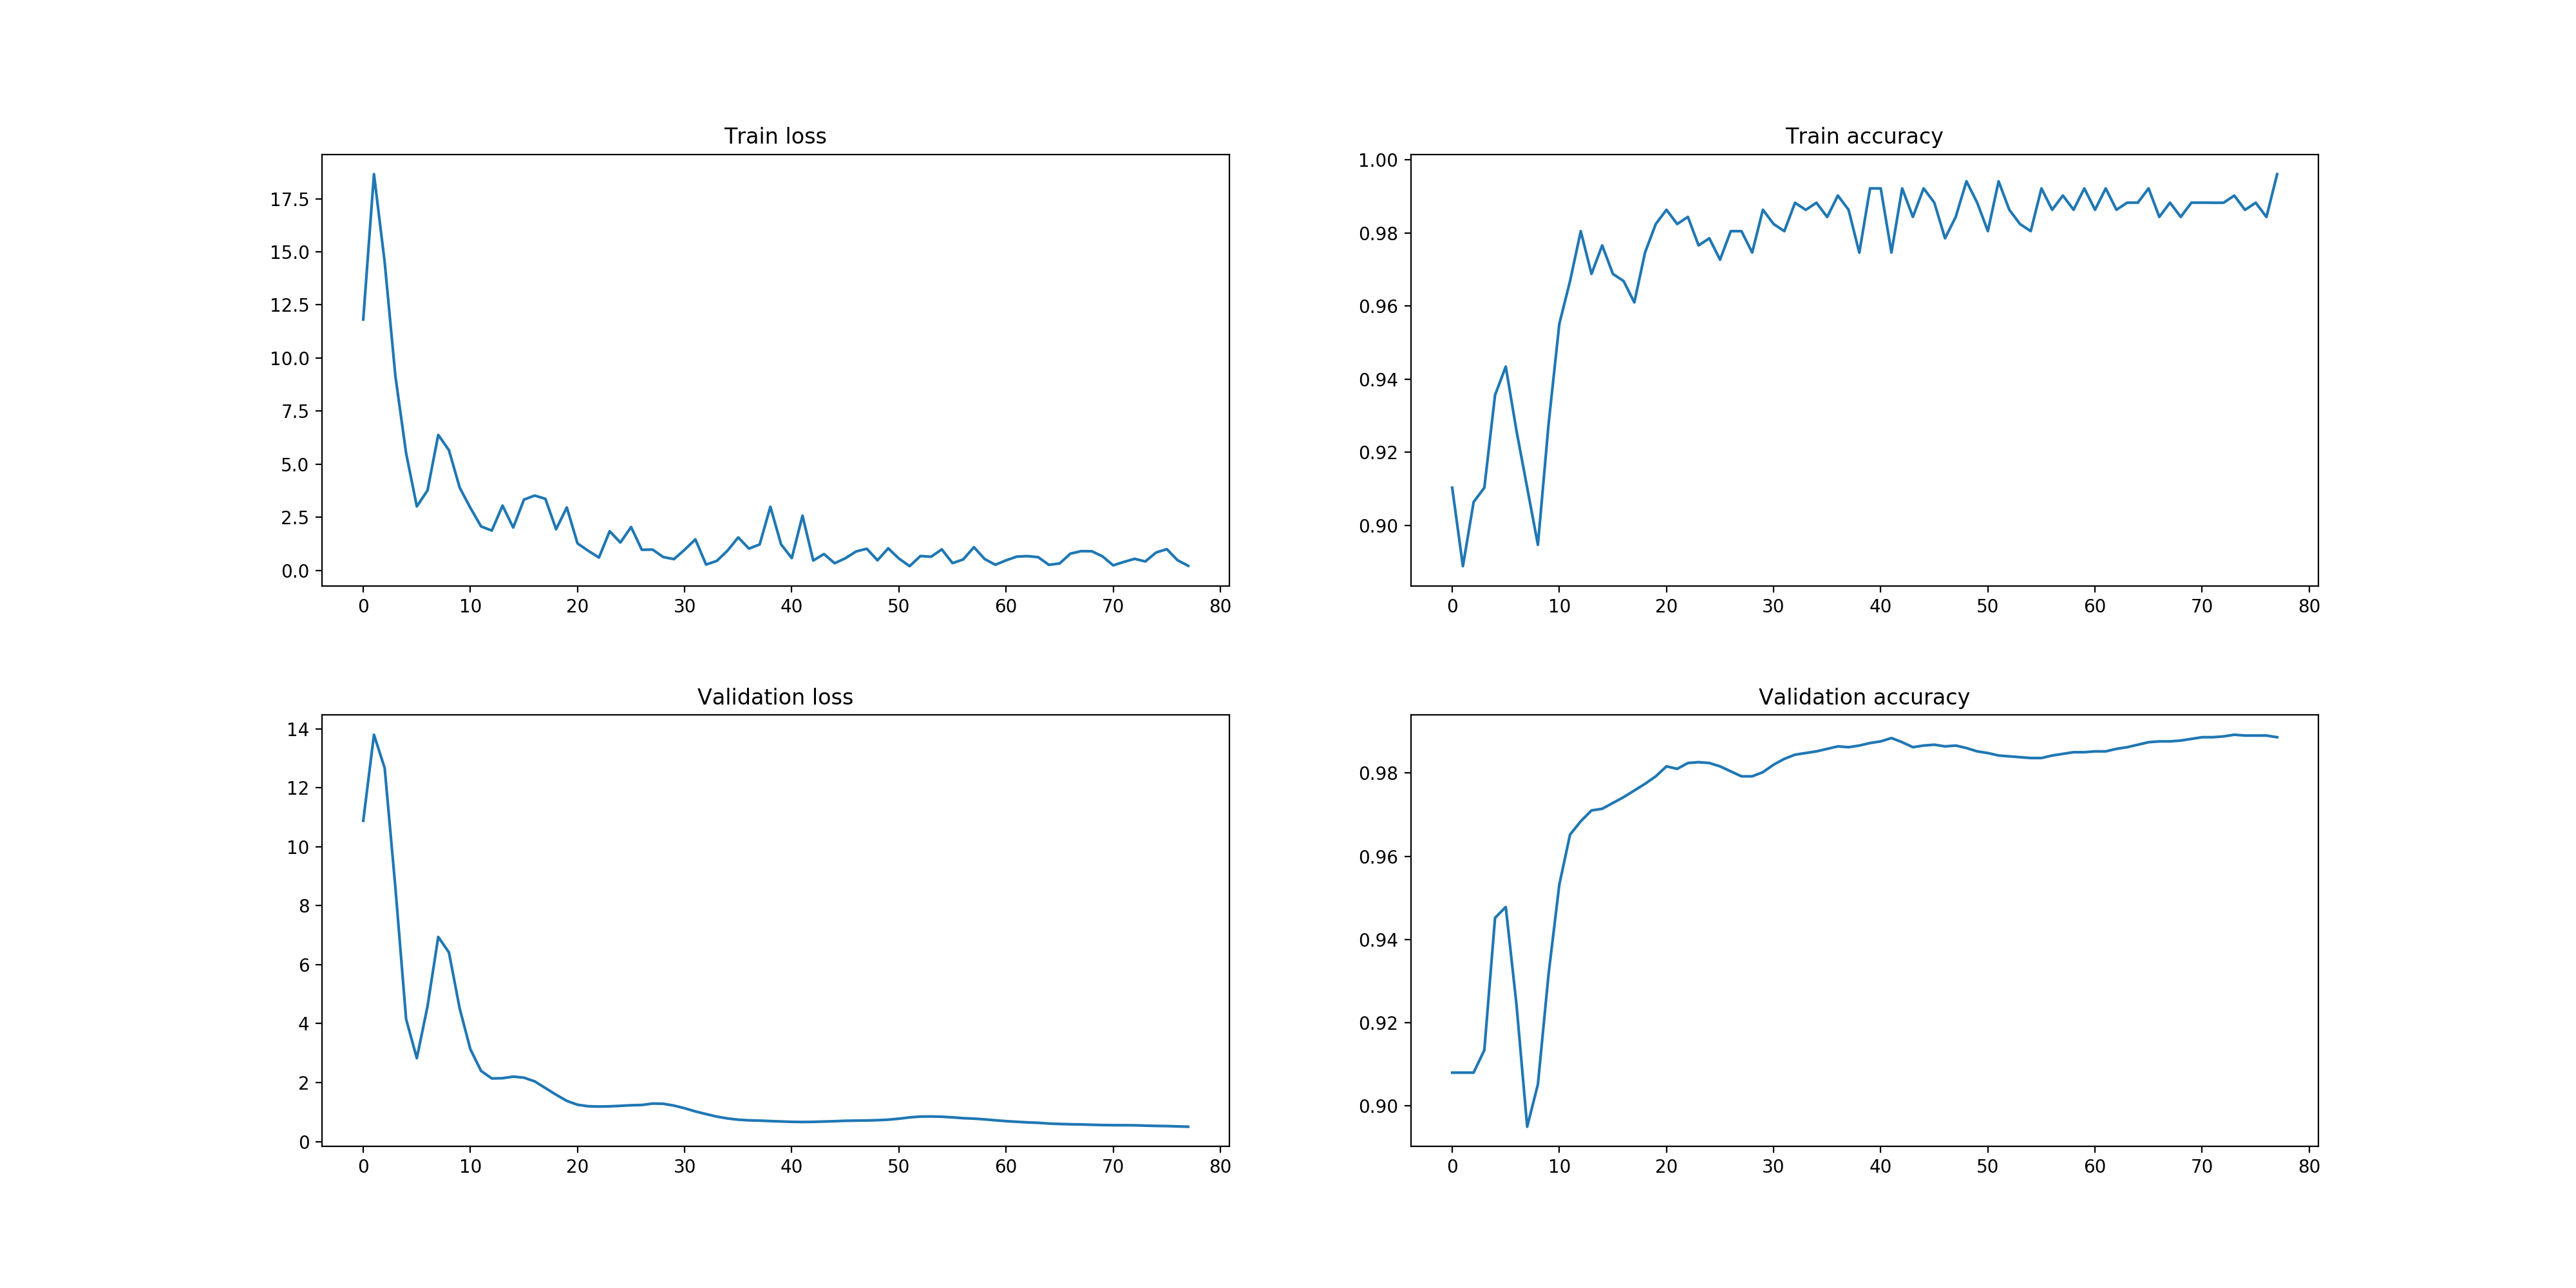
\includegraphics[scale=0.35]{../gdsvm/exports/adam_train.png}
		\caption{Erreur et précision sur MNIST pour le jeu d'entraînement et le jeu de validation}
	\end{figure}
	
	
	
	
	
	\subsection{Comparaison avec d'autres algorithmes}
	
	

	
	

\end{document}
